\documentclass[aspectratio=169]{beamer}

\mode<presentation>
{
  \usetheme{default}
  \usecolortheme{seahorse}
  \usefonttheme{professionalfonts}
  \setbeamertemplate{navigation symbols}{}
  \setbeamertemplate{caption}[numbered]
  \setbeamertemplate{footline}[frame number]
}

\usepackage[utf8x]{inputenc}
\usepackage{graphicx}
\usepackage{physics}
\usepackage{caption}
\usepackage{subcaption}
\usepackage{xcolor}
\usepackage{physics}
\usepackage{amsmath}
\usepackage{tikz}
\usetikzlibrary{positioning}
\usepackage{mathdots}
\usepackage{yhmath}
\usepackage{cancel}
\usepackage{color}
\usepackage{siunitx}
\usepackage{array}
\usepackage{multirow}
\usepackage{amssymb}
\usepackage{gensymb}
\usepackage{tabularx}
\usepackage{extarrows}
\usepackage{booktabs}
\usepackage{centernot}


\title{Online tuning of storage ring non-linear dynamics at SIRIUS and fast ORM measurement}

\author{Matheus Melo Santos Velloso \\{\small MSc. student}}

\institute{Gleb Wataghin Institute of Physics - University of Campinas\\ Accelerator Physics Group (FAC) -  Brazilian Syncrhotron Laboratory (LNLS)}

\date{Optics Tuning and Corrections for Future Colliders Workshop \\ CERN, June 2023}

\AtBeginSection[]
{
    \begin{frame}[noframenumbering,plain]
         \tableofcontents[currentsection]
   \end{frame}
}

\begin{document}
{
\setbeamertemplate{background}
{
    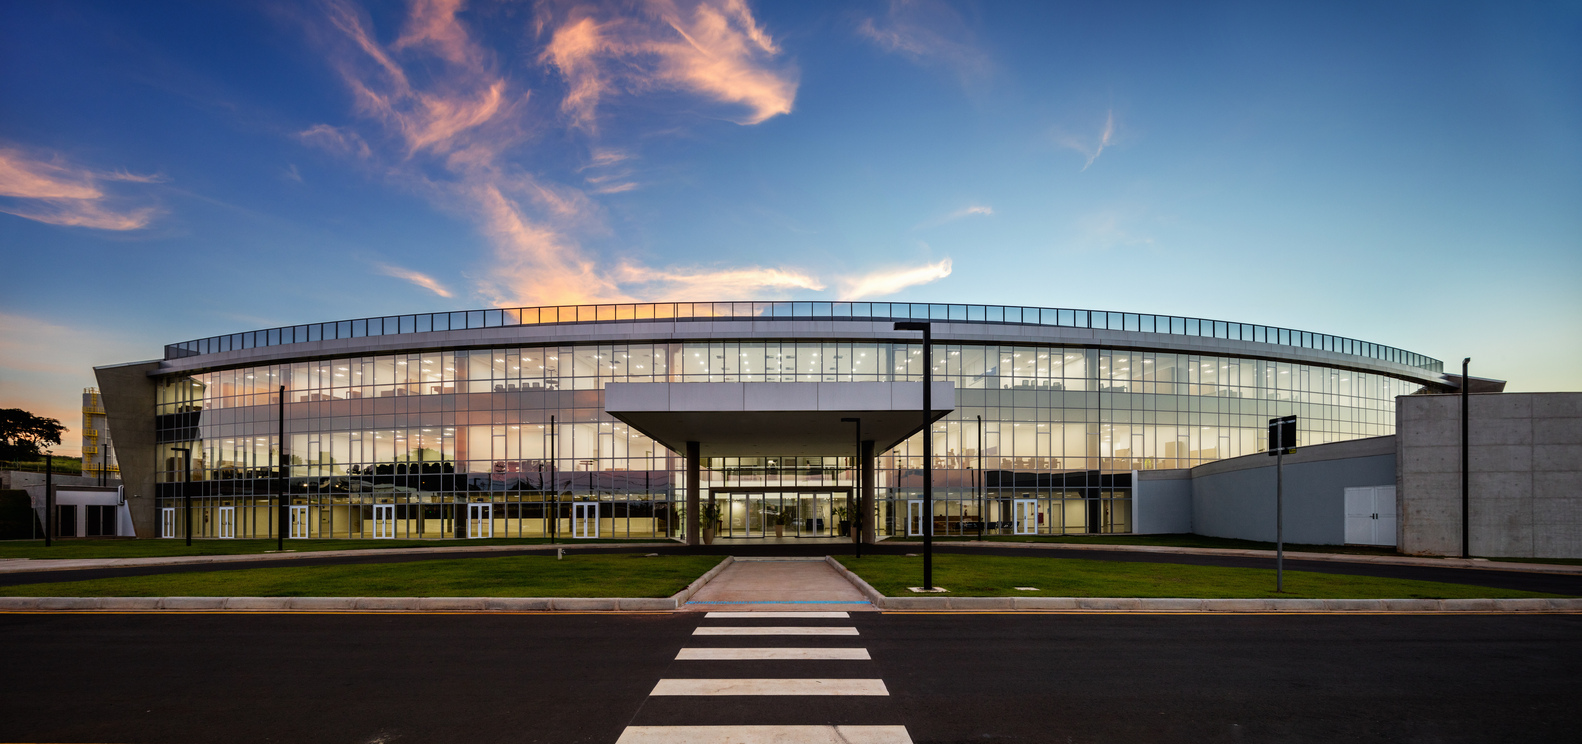
\includegraphics[width=\paperwidth, height=\paperheight]{sirius.jpg}
}
\begin{frame}[plain]
    % Title & Subtitle
    \begin{tikzpicture}[remember picture, overlay]
        \node
        [
            above=2.5cm,
            align=center,
            fill=white!20,
            inner xsep=15pt,
            inner ysep=10pt,
            minimum width=0.9\textwidth,
            text width=0.9\textwidth
        ] (title) at (current page.center)
        {
            \LARGE Online Tuning of Storage Ring Nonlinear Dynamics  \\[5pt]
            \small and Fast ORM Measruement at SIRIUS
        };

        \node[below = 0.4cm, align=center] at (title.south)
        {
        Optics Tuning and Corrections for Future Colliders Workshop \\[2pt]
        CERN, June 27, 2023
        };

        % Author
        \node
        [
            above left= 0.2cm and 0cm,
            align=right,
        ] (author) at (current page.south east)
        {
            \scriptsize \textcolor{white}{Matheus M. S. Velloso}  \\
            \tiny \textcolor{white}{Brazilian Synchrotron Light Laboratory (LNLS/CNPEM)} \\
            \tiny \textcolor{white}{Gleb Wataghin Institute of Physics (IFGW/UNICAMP)} \\
            \scriptsize \textcolor{white}{on behalf of the LNLS Accelerator Physics Group}
        };

        \node
        [
            above right =0.2cm and 0.2cm
        ] at (current page.south west)
        {
            
\includegraphics[width=3.5cm]{cnpem_lnls.png}
        };

    \end{tikzpicture}
\end{frame}
}
% \begin{frame}{Contents}
%     \tableofcontents
% \end{frame}

\section{Introduction}
\begin{frame}{SIRIUS storage ring}
    \begin{minipage}{0.35\textwidth}
        \begin{figure}
            \centering
            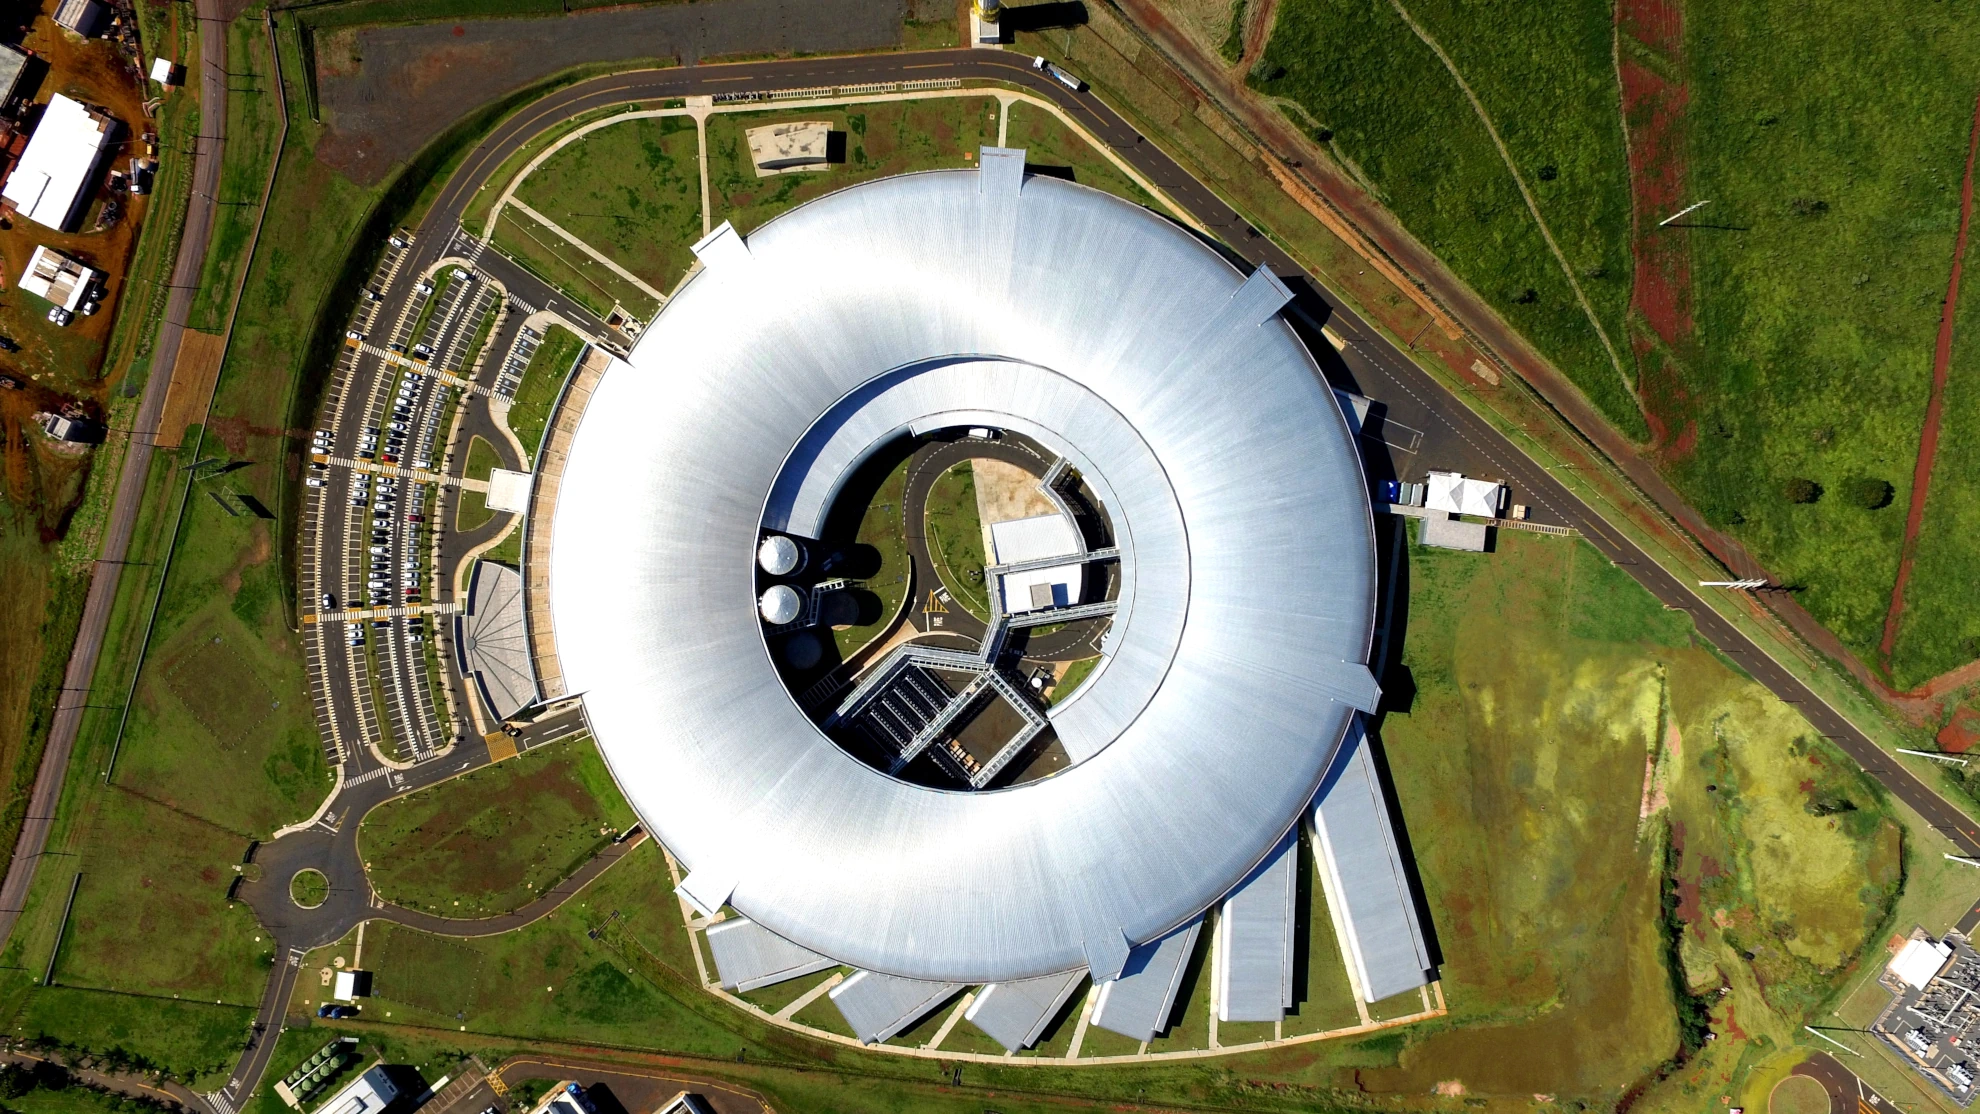
\includegraphics[angle=90, width=0.7\textwidth]{f1.png}
        \end{figure}
    \end{minipage}
    \hfill
    \begin{minipage}{0.62\textwidth}
        \scriptsize
        4th generation storage ring based Synchrotron Light Source with $250~\unit{\pico\meter~rad}$ emittance. Designed, built and operated by the Brazilian Synchrotron Light Laboratory (LNLS), at the Brazilian Center for Research in Energy and Materials (CNPEM), Campinas, Brazil.\\

        \begin{tabular}{lccc}
                \toprule\toprule
                Parameter & & Currently & Phase I \\
                \toprule
                Energy  & $E_0$  & $\SI{3}{\giga\electronvolt}$ & \\
                Current & $I_0$ &  $\SI{100}{\milli\ampere}$ & $\SI{350}{\milli\ampere}$ \\
                Operation mode & & Top-up &      \\
                Lifetime & $\tau$ & $\SI{15}{\hour}$ & $>\SI{10}{\hour}$ \\
                RF Cavities & & 1 NC & 2 SC + HC \\
                RF Voltage & $\hat{V}_{\mathrm{rf}}$ &  $\SI{1.5}{\mega\volt}$ & $\SI{3.0}{\mega\volt}$\\
                RF Frequency &   $f_{\mathrm{rf}}$ &  $\SI{499.667}{\mega\hertz}$ &  \\
                Harmonic Number &   $h$ &  864 \\
                Momentum compaction factor & $\alpha$ &   $\SI{1.6e-4}{}$ & \\
                Energy Spread & $\sigma_\delta$ &  $\SI{8.5e-4}{}$ & \\
                Bunch length & $\sigma_z$ &  $\SI{2.5}{\milli\meter}$ & $\SI{12}{\milli\meter}$ \\
                Energy loss p/ turn  & $U_0$ &  $\SI{470}{\kilo\electronvolt}$ & $\SI{870}{\kilo\electronvolt}$ \\
                % Synchrotron Tune & $\nu_z$ & $\SI{0.001638}{}$ \\
                % Frequência Síncrotron & $f_z$ &  $\SI{2.5}{\kilo\hertz}$ & \\
                % Amortecimento Longitudinal & $\tau_\delta$ &  $\SI{13}{\milli\second}$ & \\             % \\
                % \bottomrule
                % HC Type &  & Passive SC \\
                % HC RF harmonic & $q$ & 3 \\
                % HC Shunt Impedance & $R_s$ & $\SI{8.25}{\mega\ohm}$ \\
                % HC Quality Factor & $Q$ & $\SI{20800}{}$ \\
                % HC R/Q & $R/Q$ & $\SI{396}{\ohm}$ \\
                \bottomrule\bottomrule
        \end{tabular}
    \end{minipage}
\end{frame}

\begin{frame}{SIRIUS Lattice and Optics}
20$\times$5BA lattice, with 5-fold symmetric high (A) and low (B, P) betatron functions sections:  1 Superperiod = A-B-P-B
    \begin{figure}
        \centering
        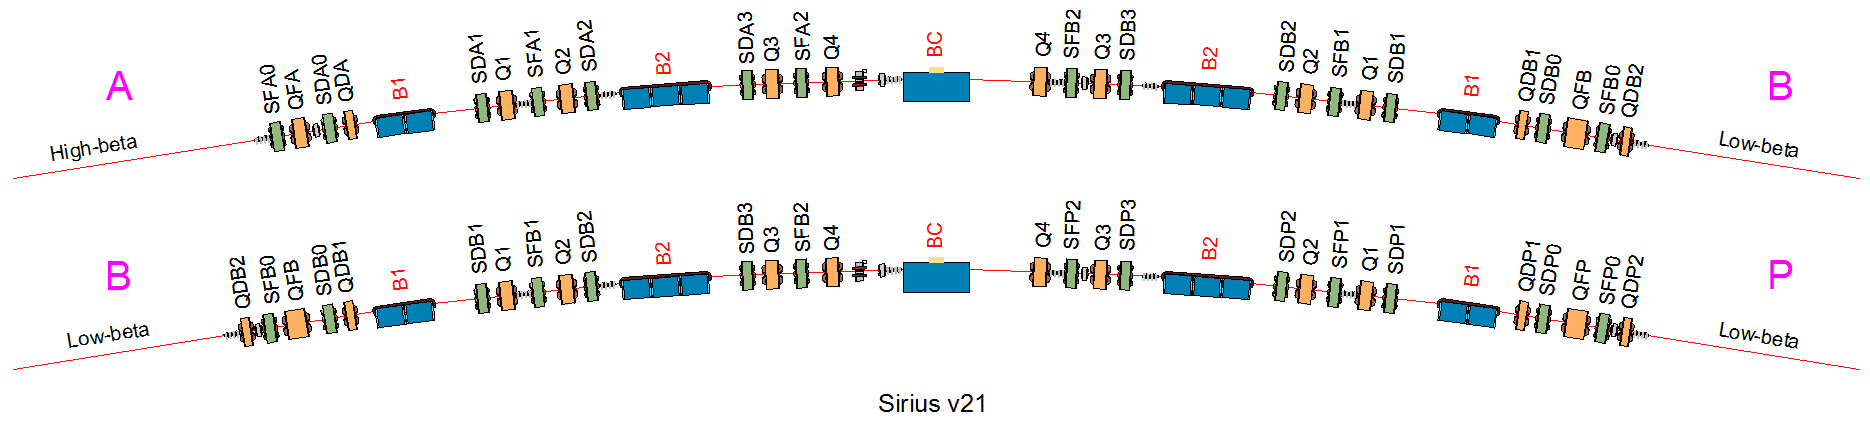
\includegraphics[width=0.8\textwidth]{SI_superperiod.png}
    \end{figure}
    \begin{figure}
        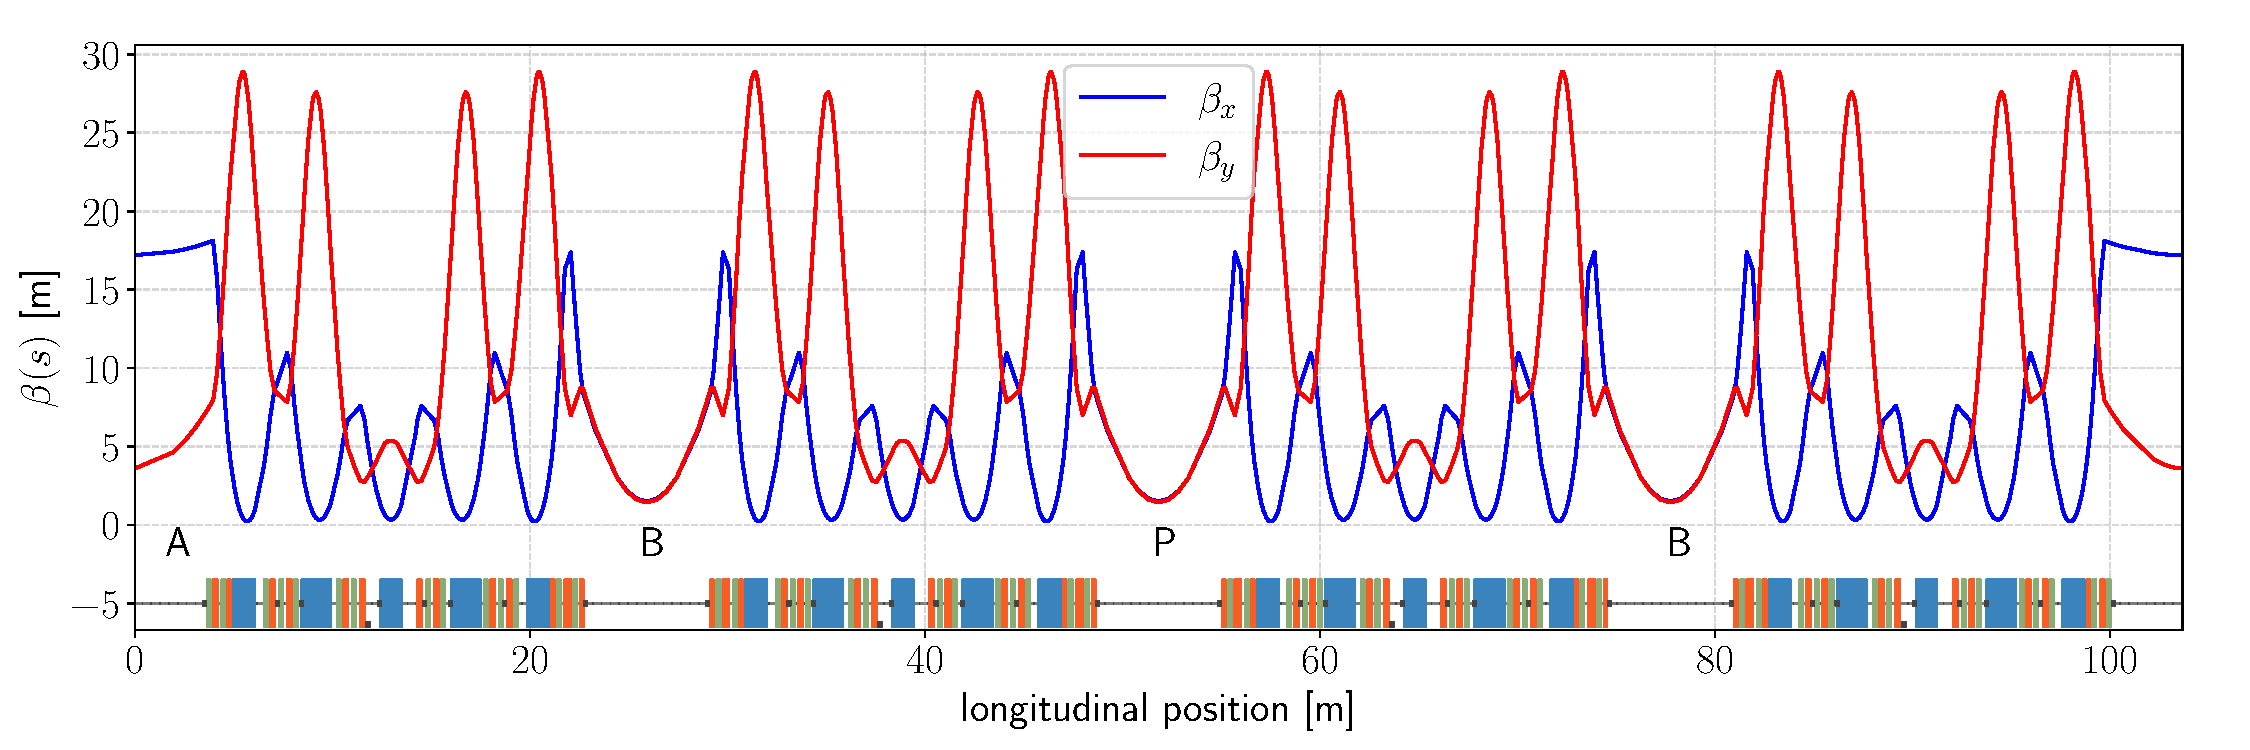
\includegraphics[width=0.8\textwidth]{beta_functions.pdf}
    \end{figure}
\end{frame}

\section{Online tuning of storage ring non-linear dynamics}
\begin{frame}{Off-axis injection scheme}
    \centering
    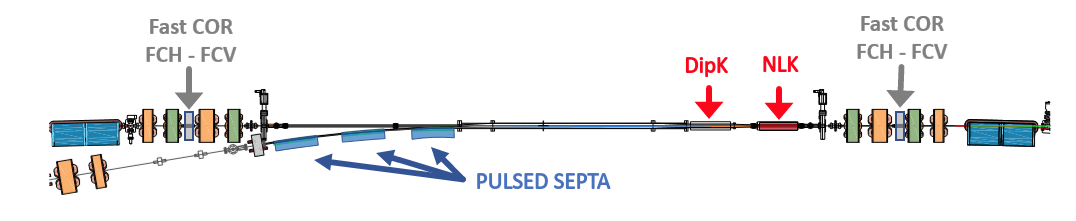
\includegraphics[width=\textwidth]{off_axis_injection.png}
    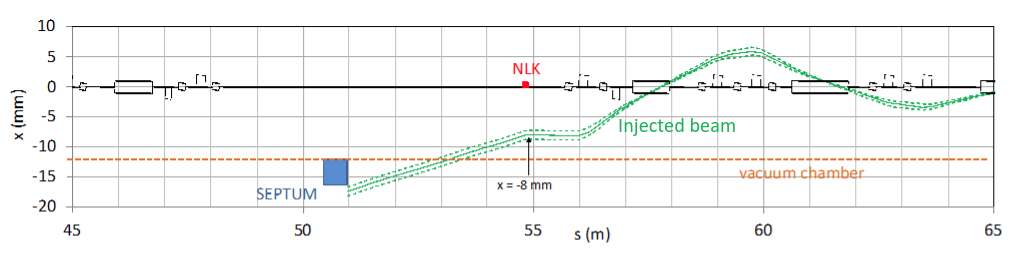
\includegraphics[width=\textwidth]{off_axis_scheme.png}
    \begin{minipage}{0.48\textwidth}
        100\% efficiency with $x=-9~\unit{mm}$ DA
    \end{minipage}
    \hfill
    \begin{minipage}{0.48\textwidth}
        88\% efficiency observed
    \end{minipage}
\end{frame}

\begin{frame}{RCDS Dynamic Aperture Optimization Setup}
    \begin{minipage}{0.6\textwidth}
        \scriptsize
        Robust conjugate direction search (RCDS) for DA optimization:
        \begin{itemize}
        \item objective function:
        \begin{itemize}
            \scriptsize
            \item avg. injection efficiency of 5 pulses @ $\unit{2~Hz}$ ($\sigma\approx1\%$)
            \item beam steered to the DA border to reduce efficiency
            \item kick resilience optimization $\centernot\implies$ injection efficiency optimization
        \end{itemize}
        \item available knobs: 21 sextupole families
        \begin{itemize}
            \scriptsize
            \item chromaticity response matrix nullspace singular-vectors (13, 17 knobs)
            \item 13 free families + 6 compensation families
        \end{itemize}
        \item  Tuning in 3 machine working points: higher fractional tunes to reduce amplification factors and improve orbit stability
        \end{itemize}
        \vfill
        \tiny
        More details:\\
        M. M. S. Velloso, M. B. Alves,  L. Liu, X. R. Resende, F. H. de Sá, and X. Huang, in \emph{Proc. IPAC'23} Venezia, 05 2023, pp. 3222-3226. WEPL087 paper\\
        {\tiny About RCDS:\\
        X. Huang, J. Corbett, J. Safranek, J. Wu, \emph{Nucl. Instr. Meth.}, vol 726, pp.77-83, 2013.\\
        X. Huang, J. Safranek, \emph{Phys. Rev. ST Accel. Beams}, vol 18, p.18}
    \end{minipage}
    \begin{minipage}{0.39\textwidth}
        \centering
        SIRIUS sextupole families
        \begin{table}[]
            \begin{tabular}{cl}
            \hline
            achromatic & \begin{tabular}[c]{@{}l@{}}SFA0, SDA0, \\ SFB0, SDB0,\\ SDP0, SFP0\end{tabular}                                                                \\ \hline
            chromatic  & \begin{tabular}[c]{@{}l@{}}SDA1, SFA1, \\ SDA2, SFA2, \\ SDA3,\\ SDB1, \textcolor{red}{SFB1}\\ SDB2, SFB2, \\ SDB3, \\ \textcolor{red}{SFP1}, SDP1,\\ SDP2, SFP2\\ SDP3\end{tabular} \\ \hline
            \end{tabular}
            \end{table}

        \vspace{0.5cm}
    \end{minipage}
\end{frame}
\begin{frame}{Tuning at $\nu_x = 49.08, \nu_y = 14.14$ (Working Point 1)}
    \begin{minipage}{0.56\textwidth}
        \begin{figure}
            \centering
            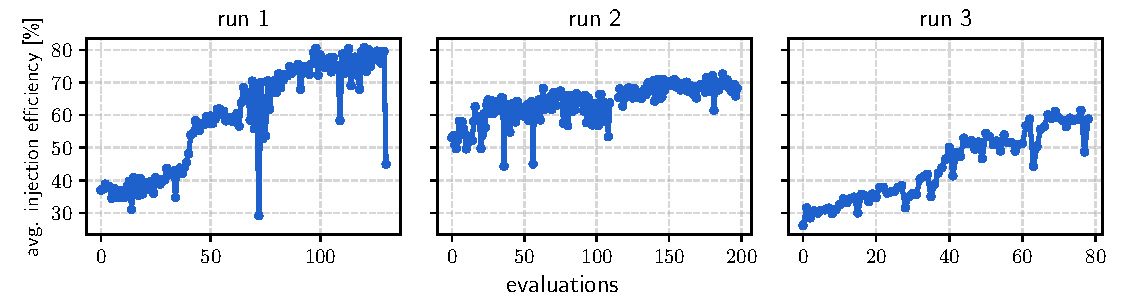
\includegraphics[width=\textwidth]{oldtunes_history.pdf}
            \pause
            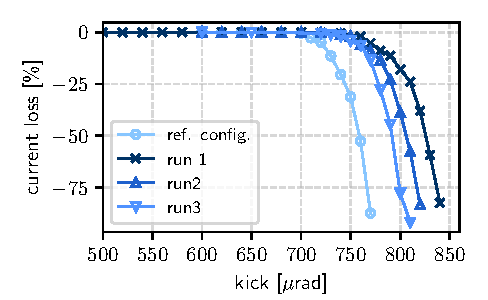
\includegraphics[width = 0.75\textwidth]{WEPL087_f1.pdf}
            \scriptsize
            \begin{table}[]
                \begin{tabular}{ccc}
                \hline
                configuration & injection efficiency $[\%]$ & lifetime @ $\unit{60~\milli\ampere}$ \\ \hline
                ref-config    & $88\pm8$                    & 21 hrs    \\
                run 1         & $91\pm1$                    &           \\
                run 2         & $98\pm1$                    &  20 hrs   \\
                run 3         & $87\pm3$                    &           \\ \hline
                \end{tabular}
                \end{table}
        \end{figure}
    \end{minipage}
    \hfill
    \begin{minipage}{0.42\textwidth}
        \begin{figure}
            \centering
            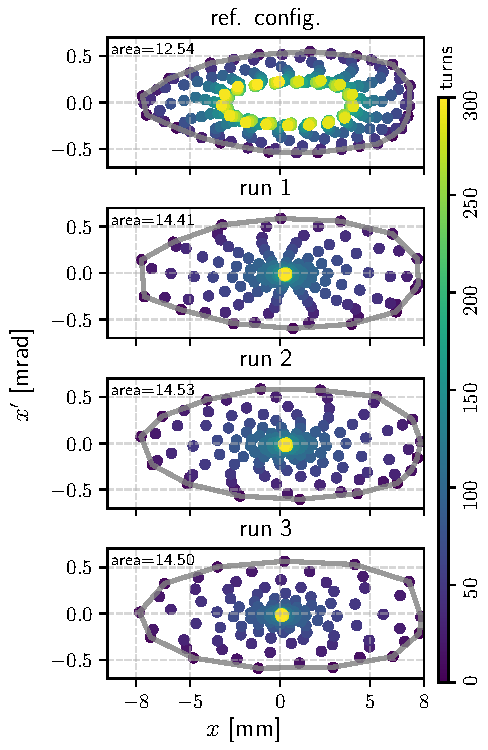
\includegraphics[height=0.9\textheight]{WEPL087_f2.pdf}
        \end{figure}
    \end{minipage}
\end{frame}
\begin{frame}{Tuning at $\nu_x = 49.20, \nu_y = 14.25$ (Working Point 2)}
    \begin{minipage}{0.55\textwidth}
        \begin{figure}
            \centering
            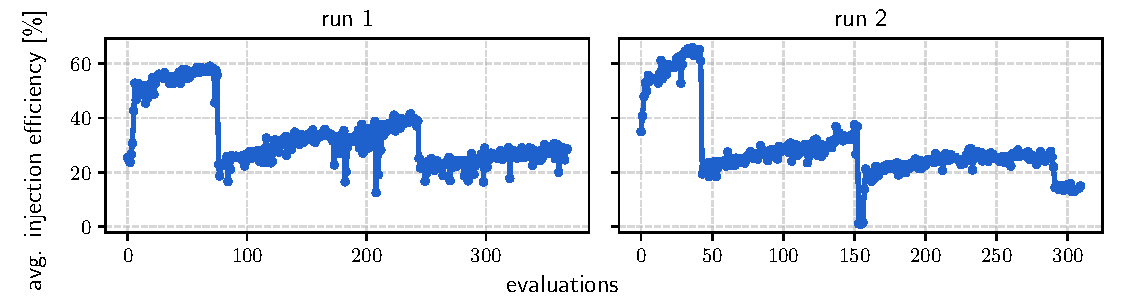
\includegraphics[width=\textwidth]{newtunes_history.pdf}
            \pause
            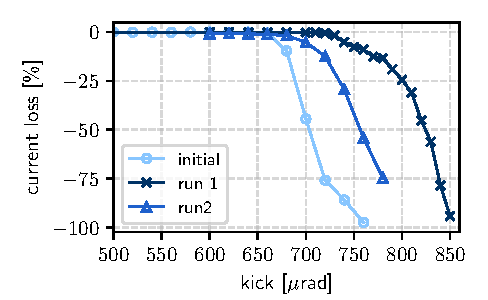
\includegraphics[width = 0.75\textwidth]{WEPL087_f3.pdf}
            \begin{table}[]
                \scriptsize
                \begin{tabular}{ccc}
                \hline
                configuration & injection efficiency $[\%]$ & lifetime @ $\unit{60~\milli\ampere}$ \\ \hline
                non-optimized    & $51\pm1$                 &  18 hrs \\
                run 1            & $79\pm3$                 &  21 hrs  \\
                run 2            & $65\pm1$                 &           \\ \hline
                \end{tabular}
                \end{table}
        \end{figure}
    \end{minipage}
    \hfill
    \begin{minipage}{0.44\textwidth}
        \begin{figure}
            \centering
            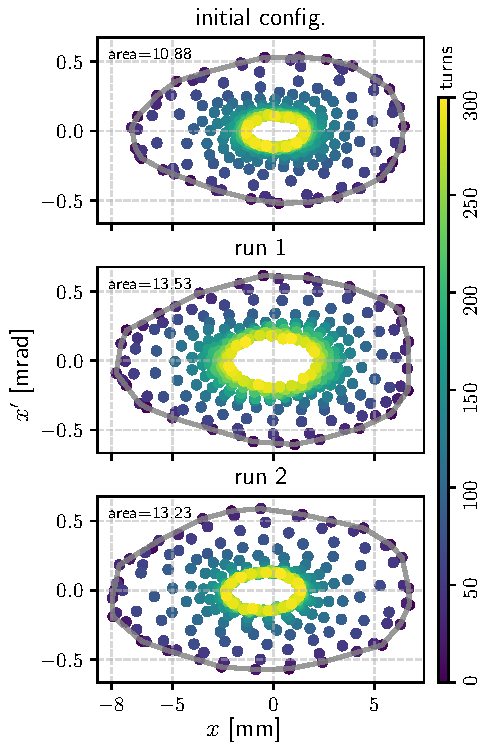
\includegraphics[height=0.9\textheight]{WEPL087_f4.pdf}
        \end{figure}
    \end{minipage}
\end{frame}
\begin{frame}{Tuning at $\nu_x = 49.16, \nu_y = 14.22$ (Working Point 3)}
    \begin{minipage}{0.55\textwidth}
        \begin{figure}
            \centering
            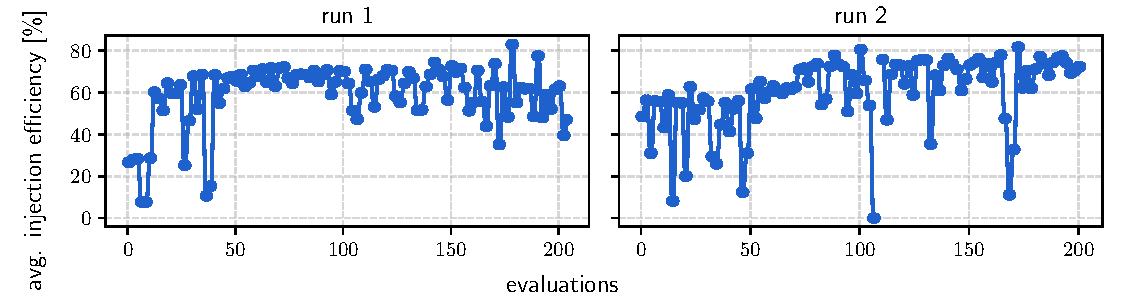
\includegraphics[width=\textwidth]{wp3_history.pdf}
            \pause
            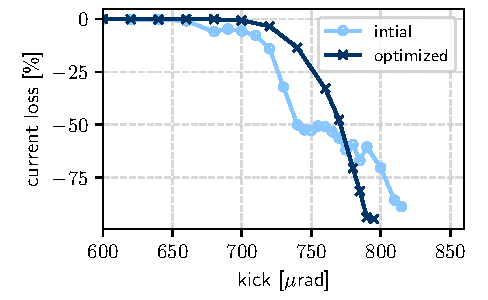
\includegraphics[width = 0.75\textwidth]{wp3_kick_resilience.pdf}
            \begin{table}[]
                \scriptsize
                \begin{tabular}{ccc}
                \hline
                configuration & injection efficiency $[\%]$  & lifetime @ $\unit{60~\milli\ampere}$  \\ \hline
                non-optimized        &                       &          \\
                optimized            & $93\pm3$              &    19.5 hrs   \\ \hline
                \end{tabular}
                \end{table}
        \end{figure}
    \end{minipage}
    \hfill
    \begin{minipage}{0.44\textwidth}
        \begin{figure}
            \centering
            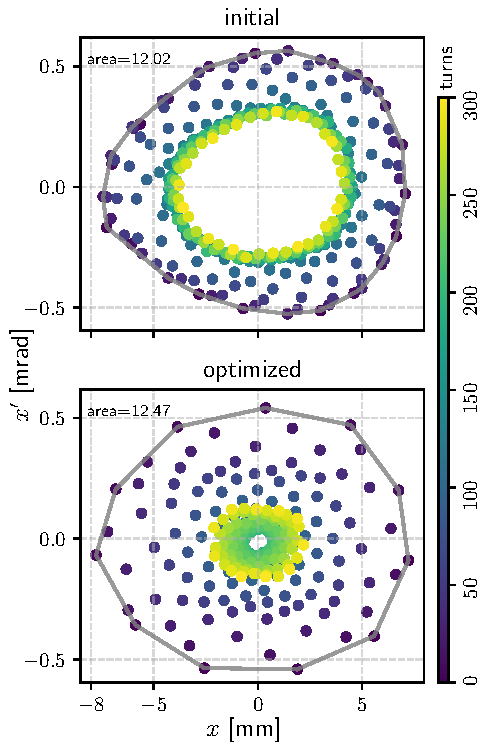
\includegraphics[height=0.9\textheight]{wp3_phase_space.pdf}
        \end{figure}
    \end{minipage}
\end{frame}

\begin{frame}{Orbit stability improvements}
WP 3 contributed for SIRIUS recent achievement of reaching $<1\%~\sigma_x$ and $<4\%~\sigma _y$ orbit rms variations in the horizontal and vertical planes, respectively.\\
\vfill
\begin{minipage}{0.7\textwidth}
    \begin{figure}
        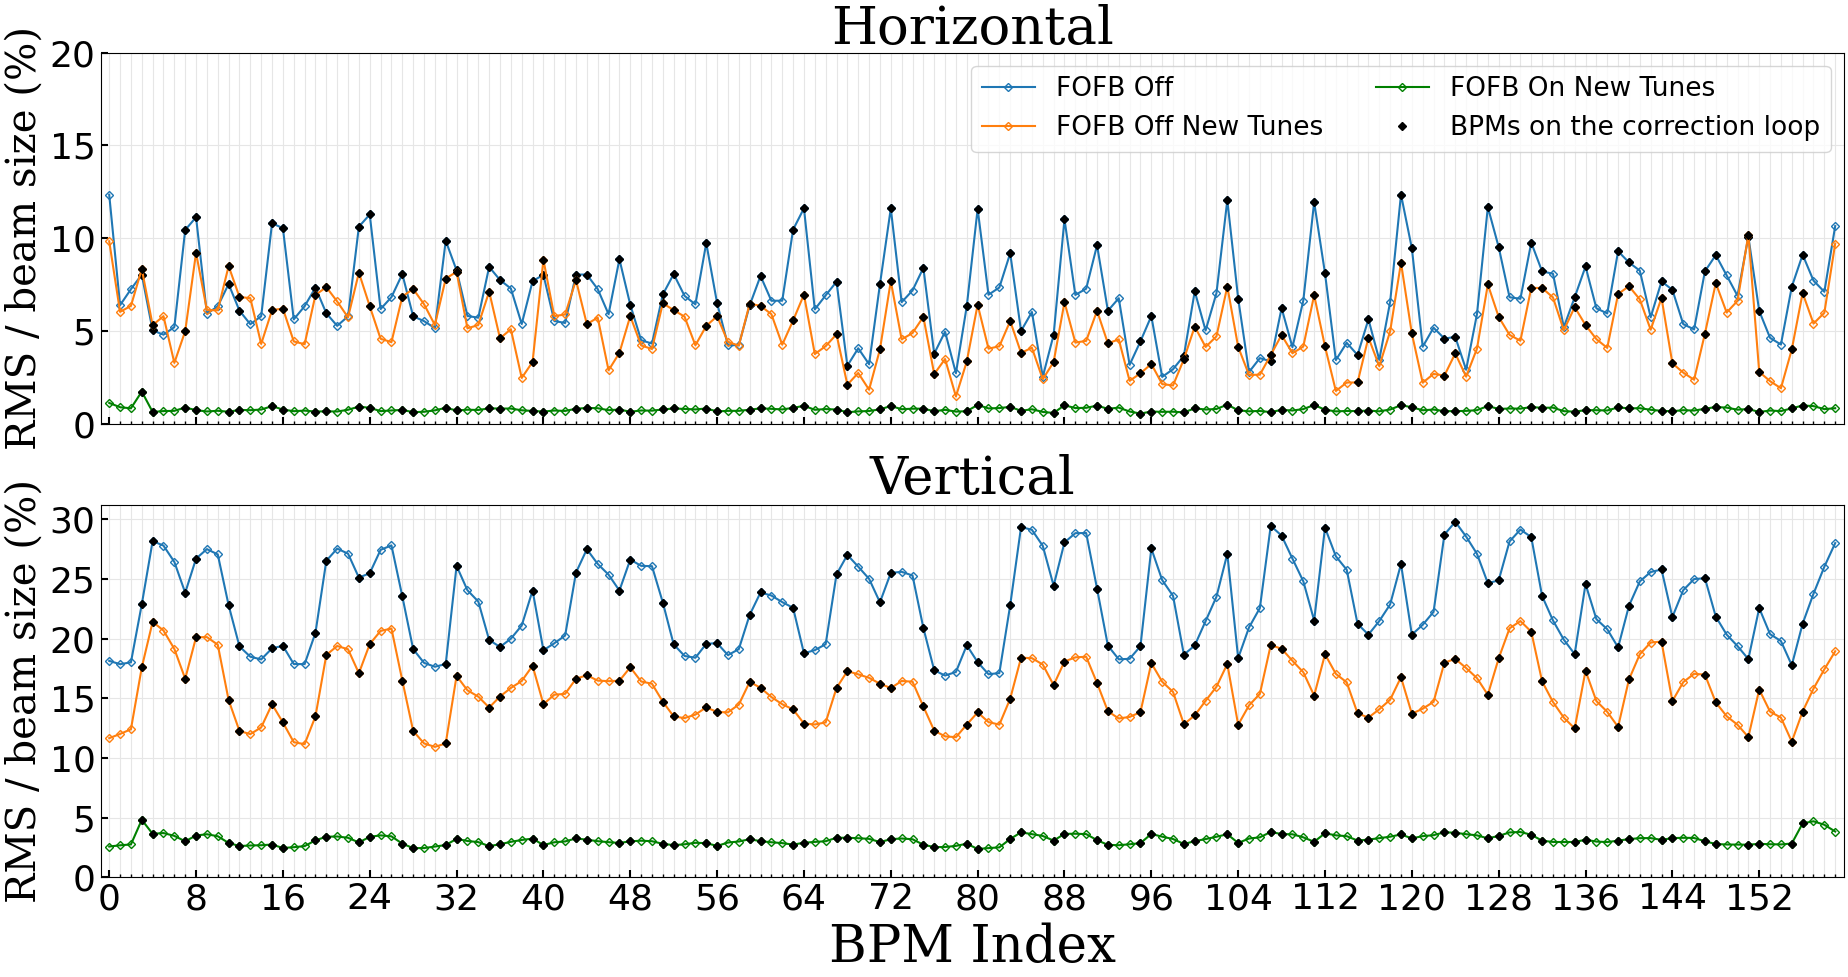
\includegraphics[width=0.9\textwidth]{WEOGA2_f5.png}
            \begin{flushleft}
            \tiny Courtesy of Daniel Tavares
        \end{flushleft}
    \end{figure}
\end{minipage}
\hfill
\begin{minipage}{0.29\textwidth}
    \scriptsize
    L. Liu \emph{et al}., “Status of SIRIUS operation with users”,
presented at the IPAC’23, Venice, Italy, May 2023, paper
WEOGA2.
\end{minipage}
\end{frame}
\begin{frame}{Summary}
    \begin{itemize}
    \item Online tuning with RCDS was effective at optimizing injection efficiency
    \item  Optimizing injection efficiency $\centernot\implies$ larger kick resiliency/larger phase portrait areas
\end{itemize}

\end{frame}

\section{Fast (``AC") Measurement of Orbit Response Matrix}
\begin{frame}{AC ORM Measurement}
    \begin{minipage}{0.44\textwidth}
        \begin{figure}
            \centering
            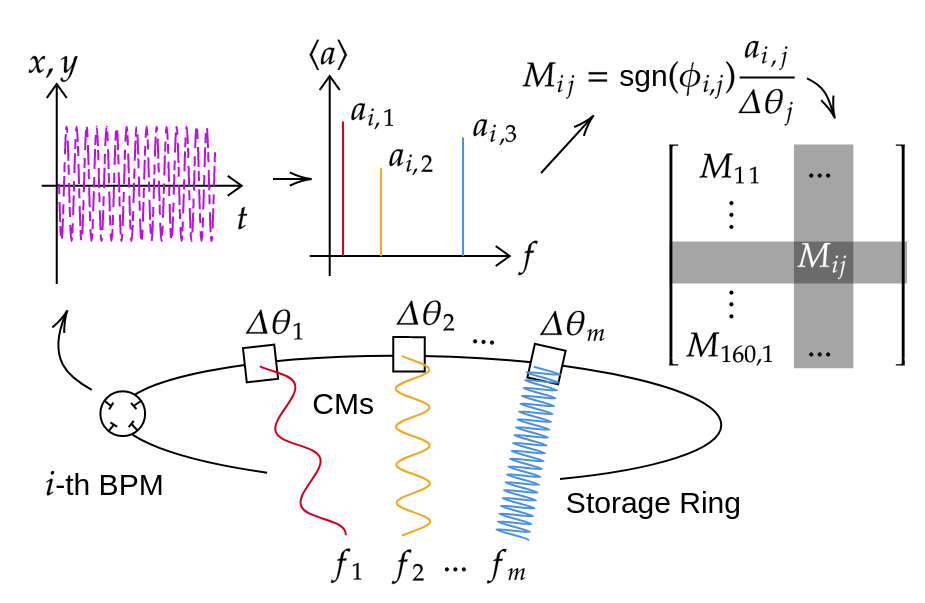
\includegraphics[width=\textwidth]{MOPOTK002_f1.png}
        \end{figure}
        \tiny
        M.M.S. Velloso, M.B. Alves, and F.H. de Sá,
   \textquotedblleft{Fast Orbit Response Matrix Measurement via Sine-Wave Excitation of Correctors at SIRIUS}\textquotedblright, in \emph{Proc. IPAC'22}, Bangkok, Thailand, Jun. 2022, pp. 425--428.
    \end{minipage}
    \begin{minipage}{0.55\textwidth}
        \begin{itemize}
            \scriptsize
            \item Fitting to $i$-th BPM data $u_i(t_j)$:
                \begin{equation*}
                    \begin{bmatrix}
                        \cos (2\pi f_{1} t_{1}) & \sin( 2\pi f_{1} t_{1}) & ... &\\
                        \cos (2\pi f_{1} t_{2}) & \sin (2\pi f_{1} t_{2}) & ...& \\
                        \vdots  & \vdots  & & \\
                        \cos (2\pi f_{1} t_{n}) & \sin (2\pi f_{1} t_{n}) & ... &
                        \end{bmatrix}\begin{bmatrix}
                            b_{i}{}_{1}\\
                            c_{i}{}_{1}\\
                            \vdots \\
                            b_{i}{}_{m}\\
                            c_{i}{}_{m}
                        \end{bmatrix} =\begin{bmatrix}
                            u_{i}( t_{1})\\
                            u_{i}( t_{2})\\
                            \vdots \\
                            u_{i}( t_{n})
                        \end{bmatrix}
                \end{equation*}
            \item Expected beam motion $$\Delta u_i(t_n) = \sum_j a_{i,j}\sin(2\pi f_j t_n + \phi_{i,j})$$
                \begin{equation*}
                    a_{i,j}=\sqrt{b^2_{i,j}+c^2_{i,j}}, \quad \phi_{i,j}=\text{atan}2(b_{i,j},c_{i,j})\in(-\pi,\pi]
                \end{equation*}
            \item ORM elements:
                \begin{equation*}
                    M_{ij}=\text{sgn}(\phi_{i,j})\frac{a_{i,j}}{\Delta \theta_j},
                \end{equation*}
        \end{itemize}
    \end{minipage}
\end{frame}
\begin{frame}{Measurements at SIRIUS storage ring}
    \begin{minipage}{0.49\textwidth}
        \scriptsize
        SIRIUS BPMs-CMs circuit
        \begin{itemize}
            \item 160 BPMs
            \item $n_x = 120$ CHs, $n_y=160$ CVs, $n=n_x+n_y=280$ CMs
        \end{itemize}
        \pause
        Measurement Procedure
        \begin{itemize}
            \item At each one of the \textbf{20 sectors},
            \begin{itemize}
            \scriptsize
            \item \textbf{6 CHs} $f_x = 3,  7, 13, 19, 29, 37\ \unit{Hz}$
            \item \textbf{8 CVs} $f_y = 5, 11, 17, 23, 31, 41, 47, 59\ \unit{Hz}$
            \item prime frequencies to easily distinguish nonlinear harmonics
            \item $\unit{5~\micro rad}$ strength, during $\unit{4~seconds}$.
            \item integer number of oscillations, orthogonal harmonics
            \end{itemize}
            \item  The complete measurement
            \begin{itemize}
                \scriptsize
                \item 30 mins for DC method
                \item $2.5-3\ \unit{mins}$ AC method
            \end{itemize}
        \end{itemize}
    \pause
    % AC- and DC-ORM signature correlation
    % \pause
    % \begin{itemize}
    %     \scriptsize
    %     \item $\cos\theta_j = \vb{v}_{\text{AC}, j}\centerdot \vb{v}_{\text{DC}, j}/\norm{\vb{v}_{\text{AC}, j}}\norm{\vb{v}_{\text{DC}, j}}$
    %     \item avg $|1 - \cos\theta_j|\sim0.03\%$ for diagonal blocks and $\sim3\%$ for off-diagonal blocks
    % \end{itemize}
    \end{minipage}
    \pause
    \hfill
    \begin{minipage}{0.49\textwidth}
        \centering
        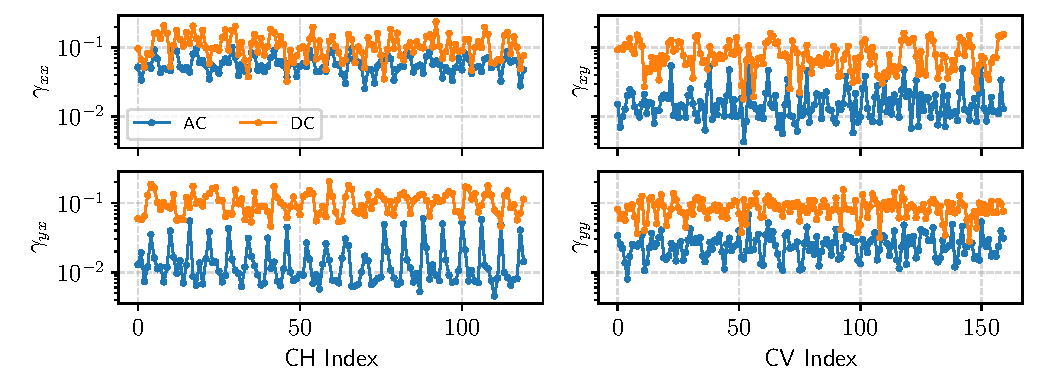
\includegraphics[width=\textwidth]{MOPOTK002_f4.pdf}
        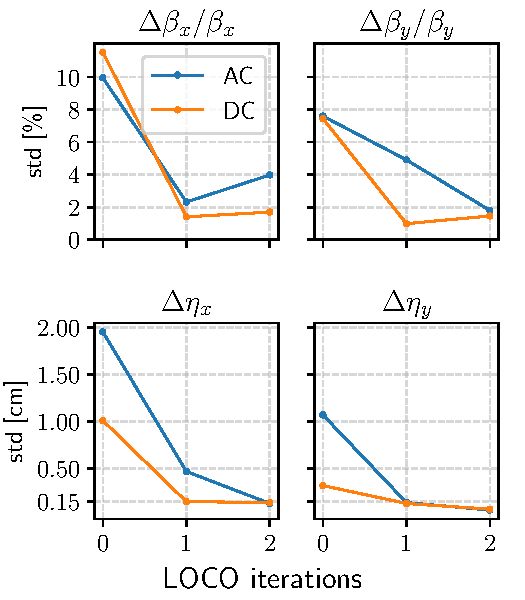
\includegraphics[height=0.6\textheight]{MOPOTK002_f5.pdf}
    \end{minipage}
\end{frame}
\begin{frame}[plain, noframenumbering]
    Thank you!\\
    \vfill
    \url{matheus.velloso@lnls.br}\\
    \vfill
    \begin{figure}
        \centering
        \scriptsize
        M. M. S. Velloso is supported by the São Paulo Reseach Foundation (FAPESP) via Grant \#2022/04162-4
        
\includegraphics[width=4cm]{fapesp.png}
    \end{figure}
    \begin{minipage}{0.49\textwidth}
        \begin{figure}
            
\includegraphics[width=6cm]{cnpem_lnls.png}
        \end{figure}
    \end{minipage}
    \begin{minipage}{0.49\textwidth}
        \begin{figure}
            
\includegraphics[width=6cm]{mcti.png}
        \end{figure}
    \end{minipage}
    \vfill
\end{frame}
\begin{frame}[noframenumbering]{Backup - AC ORM precision}
    \begin{equation*}
        \sigma_{ij}^2 = \frac{1}{N-1}\sum_{k=1}^{N}(M_{ij}^k - \ev{M}_{ij})^2, \quad 
        \gamma_j = \sqrt{\ev{\sigma_{ij}^2}_i}
    \end{equation*}
\end{frame}
\begin{frame}[noframenumbering]{Backup - NLK field profile}
    \begin{figure}
        \centering
        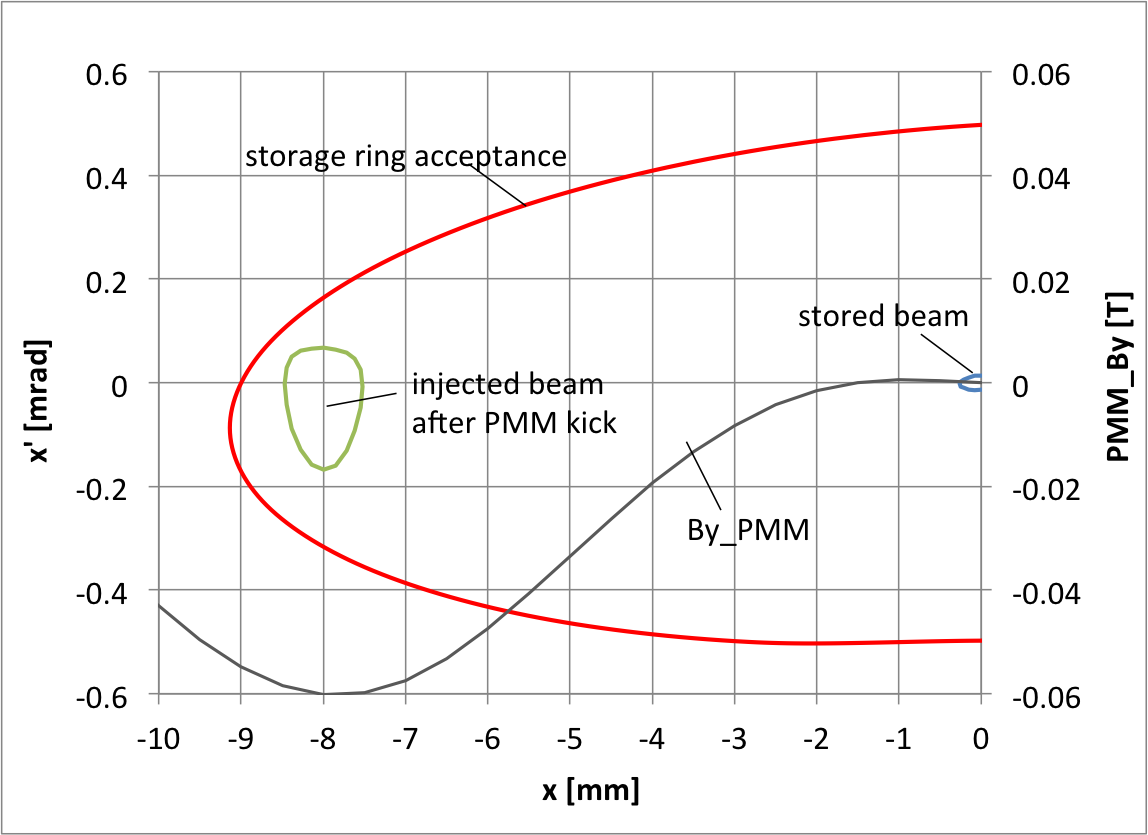
\includegraphics[width=0.7\textwidth]{nlk_phase_space.png}
    \end{figure}
\end{frame}
\end{document}
